\documentclass{article}

\usepackage{fancyhdr} % Required for custom headers
\usepackage{lastpage} % Required to determine the last page for the footer
\usepackage{extramarks} % Required for headers and footers
\usepackage[usenames,dvipsnames]{color} % Required for custom colors
\usepackage{graphicx} % Required to insert images
\usepackage{listings} % Required for insertion of code
\usepackage{courier} % Required for the courier font
\usepackage{lipsum} % Used for inserting dummy 'Lorem ipsum' text into the template
\usepackage{amsmath}
\usepackage{amssymb}
\usepackage{mathtools, xparse}
\usepackage{booktabs}
\usepackage{bigstrut}
\usepackage{float}
\usepackage{hyperref}
\usepackage{color}
\usepackage{algorithm}
\usepackage{caption}
\captionsetup{skip=0pt}
\usepackage{algpseudocode}
\usepackage{multirow}
\usepackage{subfigure}
\usepackage{longtable}
\usepackage{supertabular}

\DeclarePairedDelimiter{\norm}{\lVert}{\rVert}
\DeclarePairedDelimiter\abs{\lvert}{\rvert}%

\hypersetup{
    colorlinks   = true,    % Colours links instead of ugly boxes
    urlcolor     = red,    % Colour for external hyperlinks
    linkcolor    = red,    % Colour of internal links
    citecolor    = red      % Colour of citations
}
% Margins
\topmargin=-0.45in
\evensidemargin=0in
\oddsidemargin=0in
\textwidth=6.5in
\textheight=9.0in
\headsep=0.25in

\linespread{1.1} % Line spacing

% Set up the header and footer
\pagestyle{fancy}
\lhead{\hmwkAuthorName} % Top left header
\rhead{\hmwkClass\ : \hmwkID} % Top center head
%\rhead{\firstxmark} % Top right header
\lfoot{\lastxmark} % Bottom left footer
\cfoot{} % Bottom center footer
\rfoot{Page\ \thepage\ of\ \protect\pageref*{LastPage}} % Bottom right footer
\renewcommand\headrulewidth{0.4pt} % Size of the header rule
\renewcommand\footrulewidth{0.4pt} % Size of the footer rule
\renewcommand{\subsectionmark}[1]{\markboth{#1}{}}
\setlength\parindent{0pt} % Removes all indentation from paragraphs

%----------------------------------------------------------------------------------------
%	CODE INCLUSION CONFIGURATION
%----------------------------------------------------------------------------------------

\definecolor{MyDarkGreen}{rgb}{0.0,0.4,0.0} % This is the color used for comments
\lstloadlanguages{Perl} % Load Perl syntax for listings, for a list of other languages supported see: ftp://ftp.tex.ac.uk/tex-archive/macros/latex/contrib/listings/listings.pdf
\lstset{language=Perl, % Use Perl in this example
    frame=single, % Single frame around code
    basicstyle=\small\ttfamily, % Use small true type font
    keywordstyle=[1]\color{Blue}\bf, % Perl functions bold and blue
    keywordstyle=[2]\color{Purple}, % Perl function arguments purple
    keywordstyle=[3]\color{Blue}\underbar, % Custom functions underlined and blue
    identifierstyle=, % Nothing special about identifiers                                         
    commentstyle=\usefont{T1}{pcr}{m}{sl}\color{MyDarkGreen}\small, % Comments small dark green courier font
    stringstyle=\color{Purple}, % Strings are purple
    showstringspaces=false, % Don't put marks in string spaces
    tabsize=5, % 5 spaces per tab
    %
    % Put standard Perl functions not included in the default language here
    morekeywords={rand},
    %
    % Put Perl function parameters here
    morekeywords=[2]{on, off, interp},
    %
    % Put user defined functions here
    morekeywords=[3]{test},
    %
    morecomment=[l][\color{Blue}]{...}, % Line continuation (...) like blue comment
    numbers=left, % Line numbers on left
    firstnumber=1, % Line numbers start with line 1
    numberstyle=\tiny\color{Blue}, % Line numbers are blue and small
    stepnumber=5 % Line numbers go in steps of 5
}

% Creates a new command to include a perl script, the first parameter is the filename of the script (without .pl), the second parameter is the caption
\newcommand{\perlscript}[2]{
    \begin{itemize}
        \item[]\lstinputlisting[caption=#2,label=#1]{#1.py}
    \end{itemize}
}
\newcommand{\cppscript}[1]{
    \begin{itemize}
        \item[]\lstinputlisting[]{#1}
    \end{itemize}
}

%----------------------------------------------------------------------------------------
%	DOCUMENT STRUCTURE COMMANDS
%	Skip this unless you know what you're doing
%----------------------------------------------------------------------------------------

% Header and footer for when a page split occurs within a problem environment
\newcommand{\enterProblemHeader}[1]{
    \nobreak\extramarks{#1}{#1 continued on next page\ldots}\nobreak
    \nobreak\extramarks{#1 (continued)}{#1 continued on next page\ldots}\nobreak
}

% Header and footer for when a page split occurs between problem environments
\newcommand{\exitProblemHeader}[1]{
    \nobreak\extramarks{#1 (continued)}{#1 continued on next page\ldots}\nobreak
    \nobreak\extramarks{#1}{}\nobreak
}

%\setcounter{secnumdepth}{0} % Removes default section numbers
\newcounter{homeworkProblemCounter} % Creates a counter to keep track of the number of problems

\newcommand{\homeworkProblemName}{}
\newenvironment{homeworkProblem}[1][Problem \arabic{homeworkProblemCounter}]{ % Makes a new environment called homeworkProblem which takes 1 argument (custom name) but the default is "Problem #"
    \stepcounter{homeworkProblemCounter} % Increase counter for number of problems
    \renewcommand{\homeworkProblemName}{#1} % Assign \homeworkProblemName the name of the problem
    \section{\homeworkProblemName} % Make a section in the document with the custom problem count
    \enterProblemHeader{\homeworkProblemName} % Header and footer within the environment
    }{
    \exitProblemHeader{\homeworkProblemName} % Header and footer after the environment
}

\newcommand{\problemAnswer}[1]{ % Defines the problem answer command with the content as the only argument
\noindent\framebox[\columnwidth][c]{\begin{minipage}{0.98\columnwidth}#1\end{minipage}} % Makes the box around the problem answer and puts the content inside
}

\newcommand{\homeworkSectionName}{}
\newenvironment{homeworkSection}[1]{ % New environment for sections within homework problems, takes 1 argument - the name of the section
    \renewcommand{\homeworkSectionName}{#1} % Assign \homeworkSectionName to the name of the section from the environment argument
    \subsection{\homeworkSectionName} % Make a subsection with the custom name of the subsection
    \enterProblemHeader{\homeworkProblemName\ [\homeworkSectionName]} % Header and footer within the environment
    }{
    \enterProblemHeader{\homeworkProblemName} % Header and footer after the environment
}

%----------------------------------------------------------------------------------------
%	NAME AND CLASS SECTION
%----------------------------------------------------------------------------------------

\newcommand{\hmwkID}{hw01} % Assignment title
\newcommand{\hmwkTitle}{Displacement and Strain}
\newcommand{\hmwkDueDate}{Thursday,\ Nov\ 2,\ 2017} % Due date
\newcommand{\hmwkClass}{Principles of Biomedical Ultrasound and Photoacoustics} % Course/class
\newcommand{\hmwkClassTime}{10:30am} % Class/lecture time
\newcommand{\hmwkClassInstructor}{Jones} % Teacher/lecturer
\newcommand{\hmwkAuthorName}{106061531 Fu-En Wang} % Your name

%----------------------------------------------------------------------------------------
%	TITLE PAGE
%----------------------------------------------------------------------------------------

\title{
    \vspace{2in}
    \textmd{\textbf{\hmwkClass}}\\
    \textmd{\textbf{\hmwkID: \hmwkTitle}} \\
    \normalsize\vspace{0.1in}\small{Due\ on\ \hmwkDueDate}\\
    \vspace{3in}
}

\author{\textbf{\hmwkAuthorName}}
\date{} % Insert date here if you want it to appear below your name

%----------------------------------------------------------------------------------------

\begin{document}
\maketitle
\newpage

\section{Introduction}
For \textbf{Focused Ultrasound Thermal Therapy}, an important technique is to estimate the temperature change before and after applying it.
The estimation can be derived by the echo-time shift before and after heating. Moreover, the temperature change can be formula as:
\begin{align}
\Delta T(z) = \frac{C_0}{2} \cdot K \cdot \frac{\partial \Delta t(z)}{\partial z}
\label{eq:temp change}
\end{align}
where $\Delta T(z)$ is the temperature change, $C_0$ is the speed of sound, $K$ is a constant, $\frac{\partial \Delta t(z)}{\partial z}$
is the \textbf{thermal strain}.

In this homework, we need to finish the following requirements:
\begin{enumerate}
	\item Estimate echo time shift in $\mu s$ as a function of depth
	\item Estimate thermal strain in \% as a function of depth
\end{enumerate}

\section{Source Code}
In this zip archive, there are two matlab source code files:
\begin{enumerate}
	\item \textbf{EE6265\_HW1\_106061531.m}
	\item \textbf{Windows.m}
\end{enumerate}
"EE6265\_HW1\_106061531.m" is the main flow of this homework. It will use the class \textbf{Windows} in "Windows.m" to create
an object, which can manage each window and makes our code more elegant, and plot figures with our given parameters.

\section{Problems}
In Equation \ref{eq:temp change}, the term $\Delta t(z)$ is the echo-time shift before and after ultrasound heating. Because 
$\Delta t(z)$ is a function of $z$, which means $\Delta t(z)$ will vary at different depth. As a result, we can divide the 
pre-signal and post-signal into several frames with certain window size and apply cross-correlation for each pre/post window
pair. By this way, we can estimate the time shift for each window. For more accurate result, we can upsample the origin signal
to get more sample points and higher sample rate. In this homework, I upsample the signal to 10x origin sample rate
($10 \times f_s$) and use a moving average filter to denoise the echo-time shift.

Because sliding-window is somehow like sampling, so we can treat it as down-sample process, which will reduce sampling rate.
From this assumption, we can find a new sampling rate by
\begin{align*}
    f_s' = \frac{\text{number of windows}}{length(signal)} \cdot f_s
\end{align*}
After we have new $f_s$, we can treat echo-time shift as a signal and use FFT to analyze it. Figure \ref{fig:fft-non} shows the
FFT result. In this figure, the highest peak is located at $\pm 4.398 \cdot 10^4$ Hz, which is the part to tell us where
is the focused point of ultrasound. As a result, now our task is to design a moving average filter which cut-off frequency
is $\pm 4.398 \cdot 10^4$ Hz. By the cut-off frequency formula
\begin{align*}
    \frac{f_{cut}}{f_s} = \frac{0.442947}{\sqrt{N^2 - 1}}
\end{align*}
we can find the filter size ($N$) to design appropriate moving average filter. Figure \ref{fig:fft} shows the result FFT
result after applying moving average filter.

\begin{figure}[H]
    \centering
    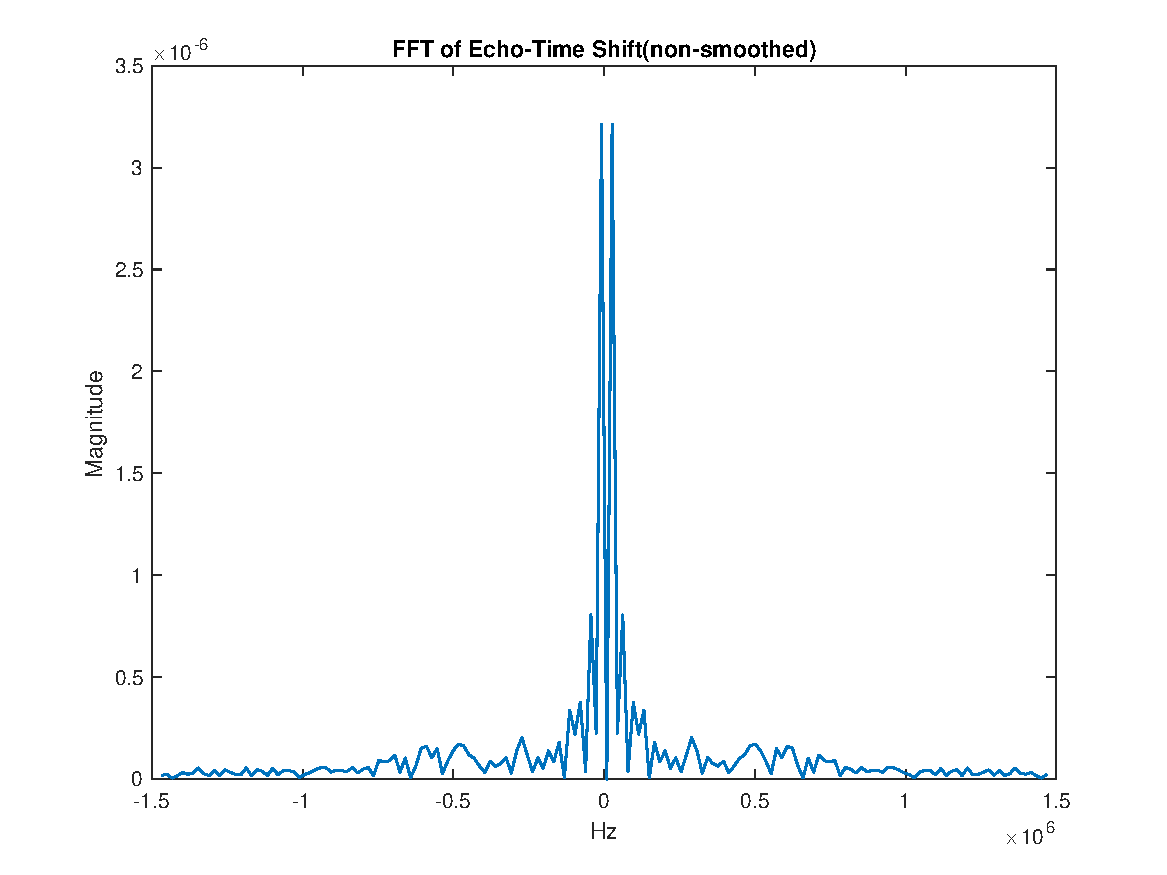
\includegraphics[width=0.8\textwidth]{src/fft_non.pdf}
    \caption{FFT of Echo-Time Shift (non-smoothed)}
    \label{fig:fft-non}
\end{figure}
\begin{figure}[H]
    \centering
    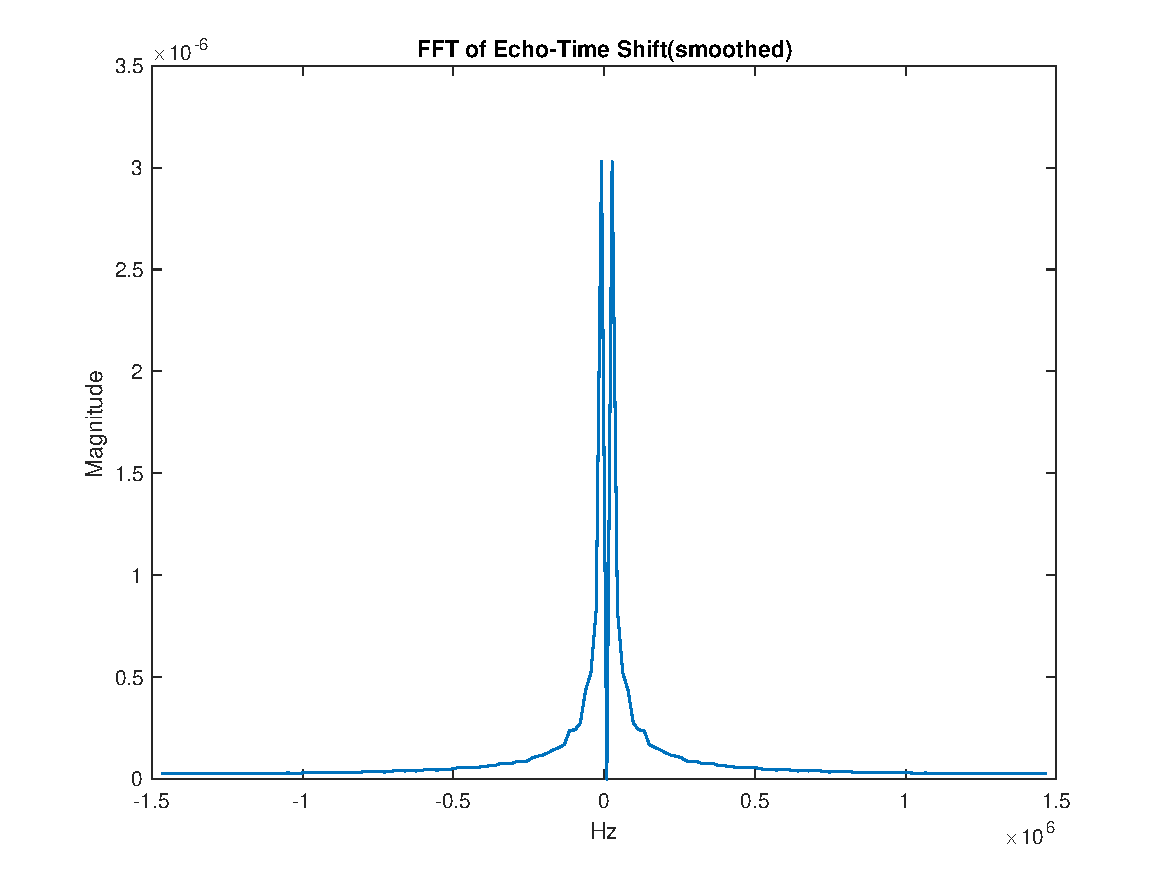
\includegraphics[width=0.8\textwidth]{src/fft.pdf}
    \caption{FFT of Echo-Time Shift (smoothed)}
    \label{fig:fft}
\end{figure}
From Figure [\ref{fig:fft-non}, \ref{fig:fft}], we can find that the highest peak is preserved and the others are well 
suppressed. Now we can move on to the next tasks, echo-time shift and thermal strain; in the following section, I will
show and explain several experiments.

\subsection{Echo-Time Shift}
In this part, I run experiments with different paramters. Windows size is 2, 6, 10 wavelength, and each combines with different 
overlap ratio (0, 0.5, 0.75). Figure [\ref{fig:shift-2}, \ref{fig:shift-6}, \ref{fig:shift-10}] show the Echo-Time Shift
as a function of $z$ for M = 2, 6 and 10, respectively.

When M=2 (Figure \ref{fig:shift-2}), echo-time shift is a little bit unstatble, which means the noise is obvious. This is because 
small window size will focus on \textbf{local information}, which make it sensitive to noise. So even if we have smoothen it, we 
still see noise on the wave. As for the overlap ratio, theoretically small ratio will drop out the variation of signal. So 
when N=0.75, we can see a more detailed change of slope.

In Figure \ref{fig:shift-6} and \ref{fig:shift-10}, the wave become quite stable because window size is getting larger. And 
when N=0.75, the result looks more realistic and its slope change more continueous.

\begin{figure}[H]
    \centering
    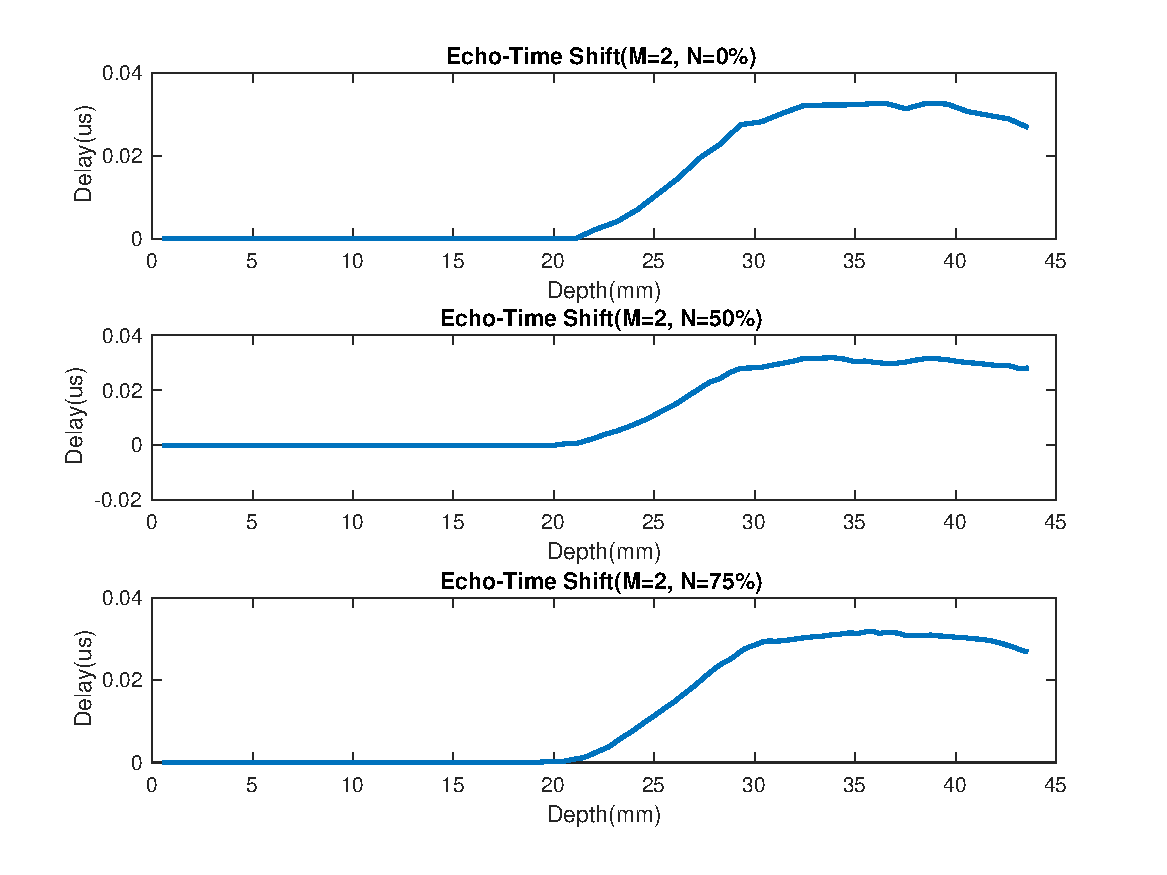
\includegraphics[width=0.82\textwidth]{src/shift_2.pdf}
    \caption{Echo-Time Shift (M=2)}
    \label{fig:shift-2}
\end{figure}
\begin{figure}[H]
    \centering
    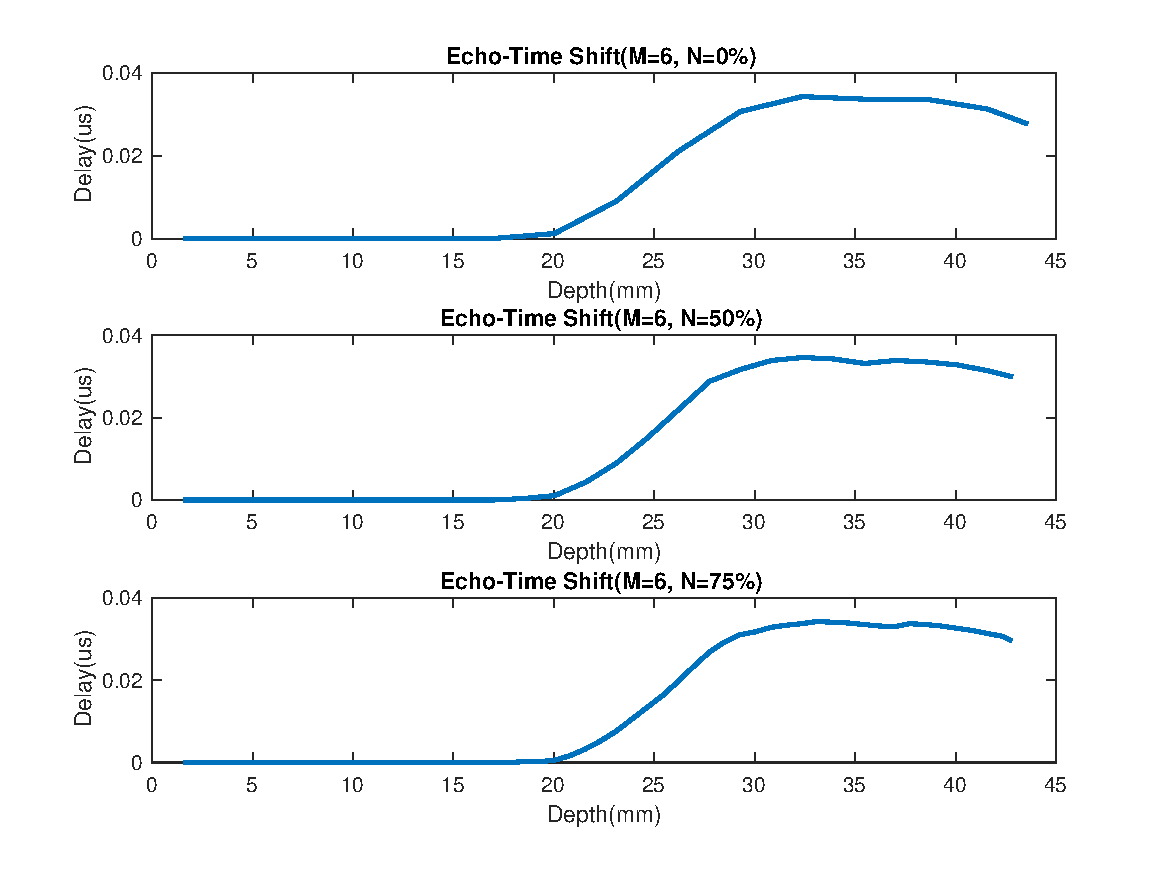
\includegraphics[width=0.82\textwidth]{src/shift_6.pdf}
    \caption{Echo-Time Shift (M=6)}
    \label{fig:shift-6}
\end{figure}
\begin{figure}[H]
    \centering
    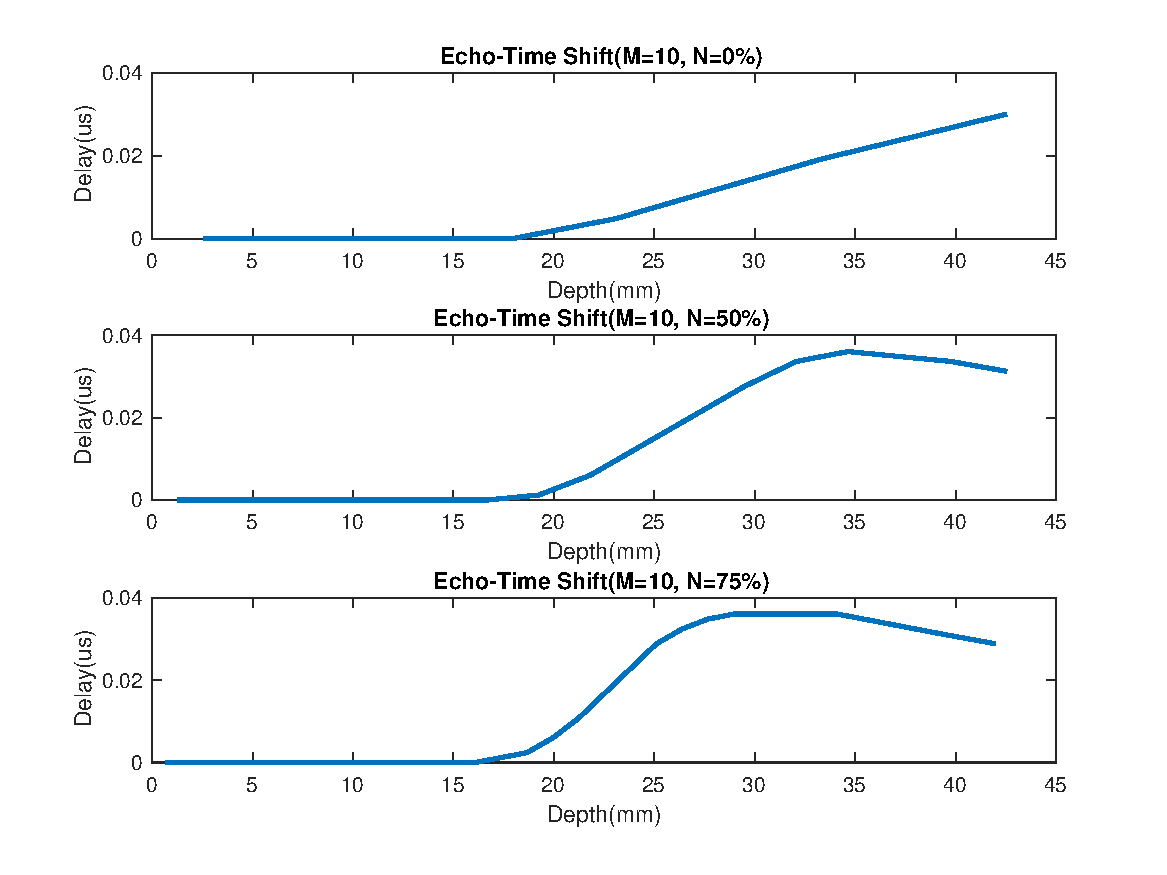
\includegraphics[width=0.82\textwidth]{src/shift_10.pdf}
    \caption{Echo-Time Shift (M=10)}
    \label{fig:shift-10}
\end{figure}

\subsection{Thermal Strain}
In this section, we need to estimate thermal strain $\frac{\partial \Delta t(z)}{\partial z}$. First, we need to convert the 
echo-time shift into distance and then use difference approximation to calculate partial differential term as shown in 
Equation \ref{eq:partial}:
\begin{align}
    \frac{\partial \Delta t(z)}{\partial z} \approx \frac{diff(\Delta t(z) \cdot \frac{C_0}{2})}{diff(Depth)}
    \label{eq:partial}
\end{align}
Figure [\ref{fig:strain-2}, \ref{fig:strain-6}, \ref{fig:strain-10}] show the Thermal Strain (\%) as a function of $z$ 
for M = 2, 6 and 10, respectively.


Because $\frac{\partial \Delta t(z)}{\partial z}$ can be treated as the slope of siganl, if the slope is unstable we will
get a bad result; in another words, derivative is very sensitive to noise. When M=2, the waveform (Figure \ref{fig:shift-2})
is unstable, so the thermal strain in Figure \ref{fig:strain-2} looks terrible. However, we can stiil find that, the maximun is
located at about 25 mm, which should be the focus point of ultrasound.

In Figure \ref{fig:strain-6}, the result looks much better because echo-time shift when M=6 (Figure \ref{fig:shift-6}) is stabler
than M=2. When N is larger, the width of lobe which is location at about 25 mm position become more narrow, which means the 
quality is better. However, we still see obvious noise at 36 mm.

In Figure \ref{fig:strain-10}, the result is better than that in Figure [\ref{fig:strain-2}, \ref{fig:strain-6}]. Because the 
window size is large enough, it is robust to noise. When N=0.75, we see a clear main lobe centered at about 25 mm. As a result,
I think (M=10, N=0.75) is the best parameters in this homework.


\begin{figure}[H]
    \centering
    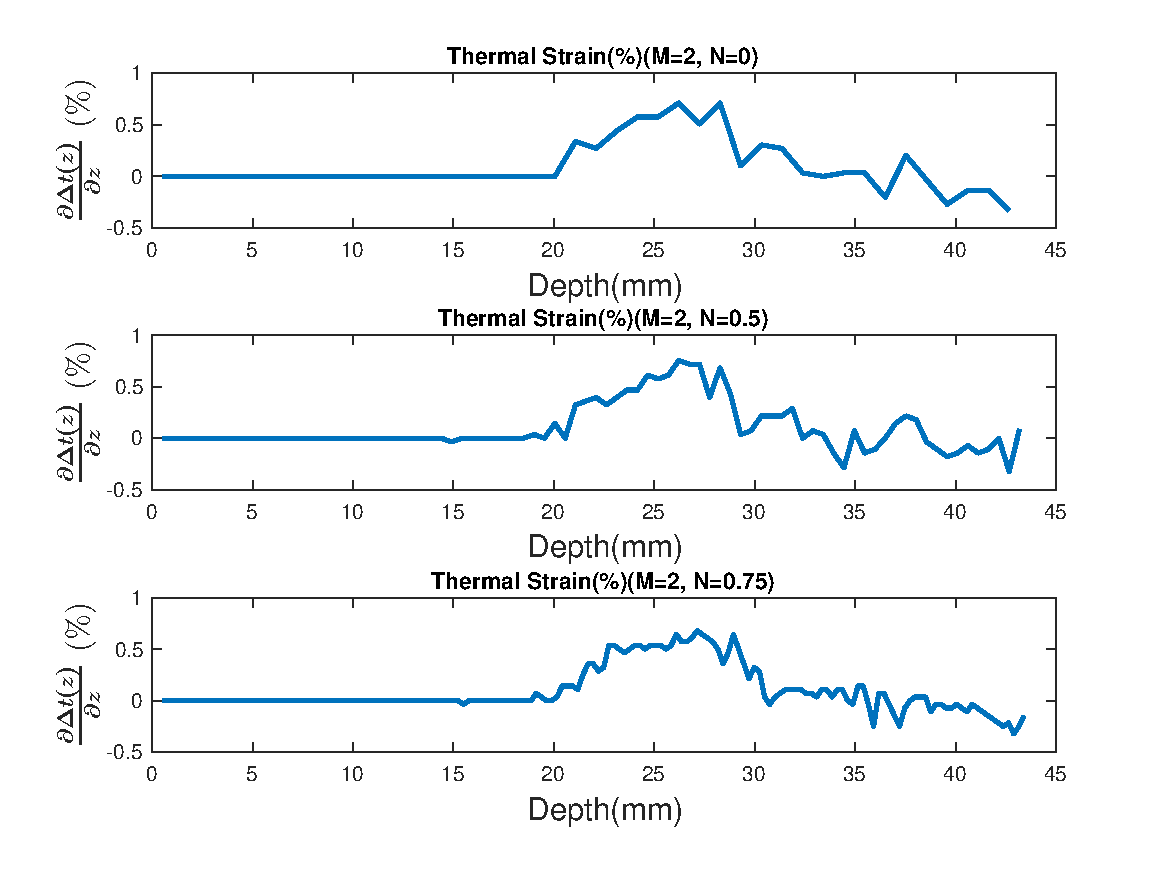
\includegraphics[width=0.82\textwidth]{src/strain_2.pdf}
    \caption{Thermal Strain (M=2)}
    \label{fig:strain-2}
\end{figure}
\begin{figure}[H]
    \centering
    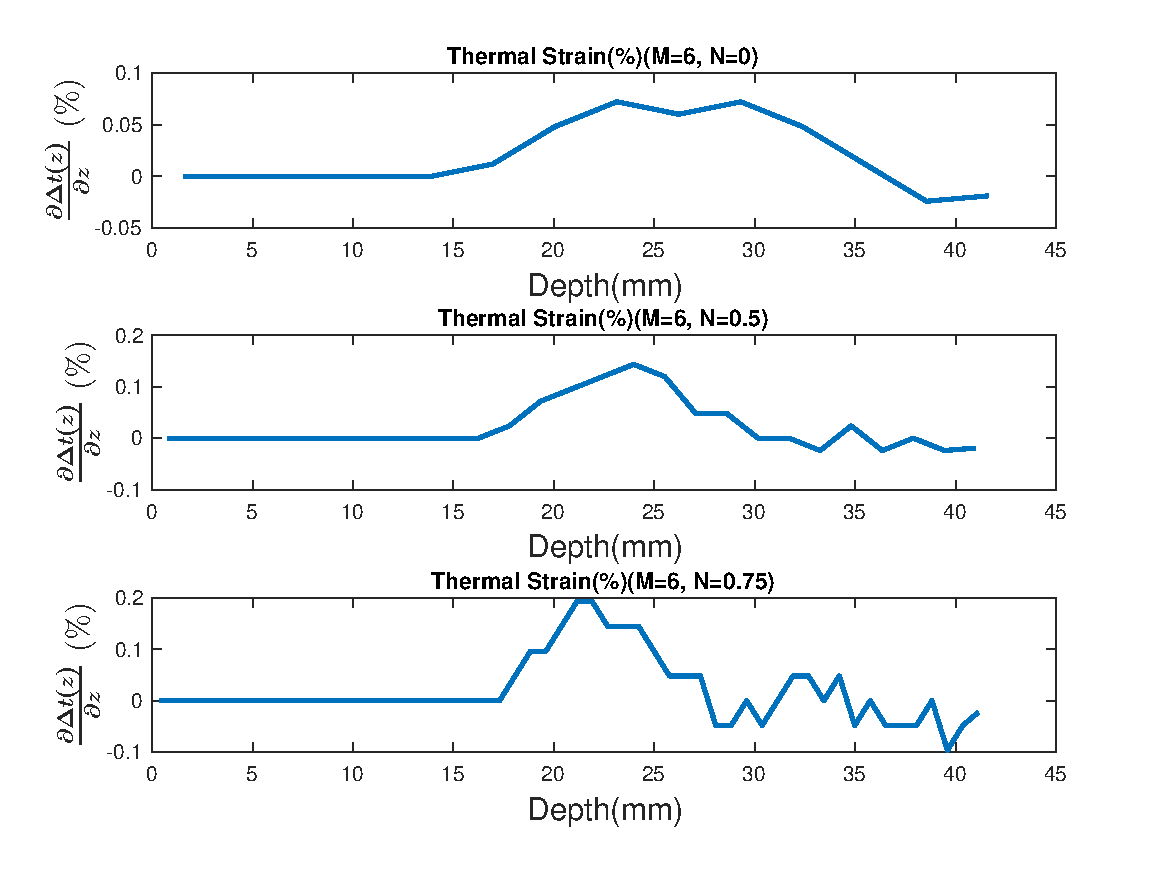
\includegraphics[width=0.82\textwidth]{src/strain_6.pdf}
    \caption{Thermal Strain (M=6)}
    \label{fig:strain-6}
\end{figure}
\begin{figure}[H]
    \centering
    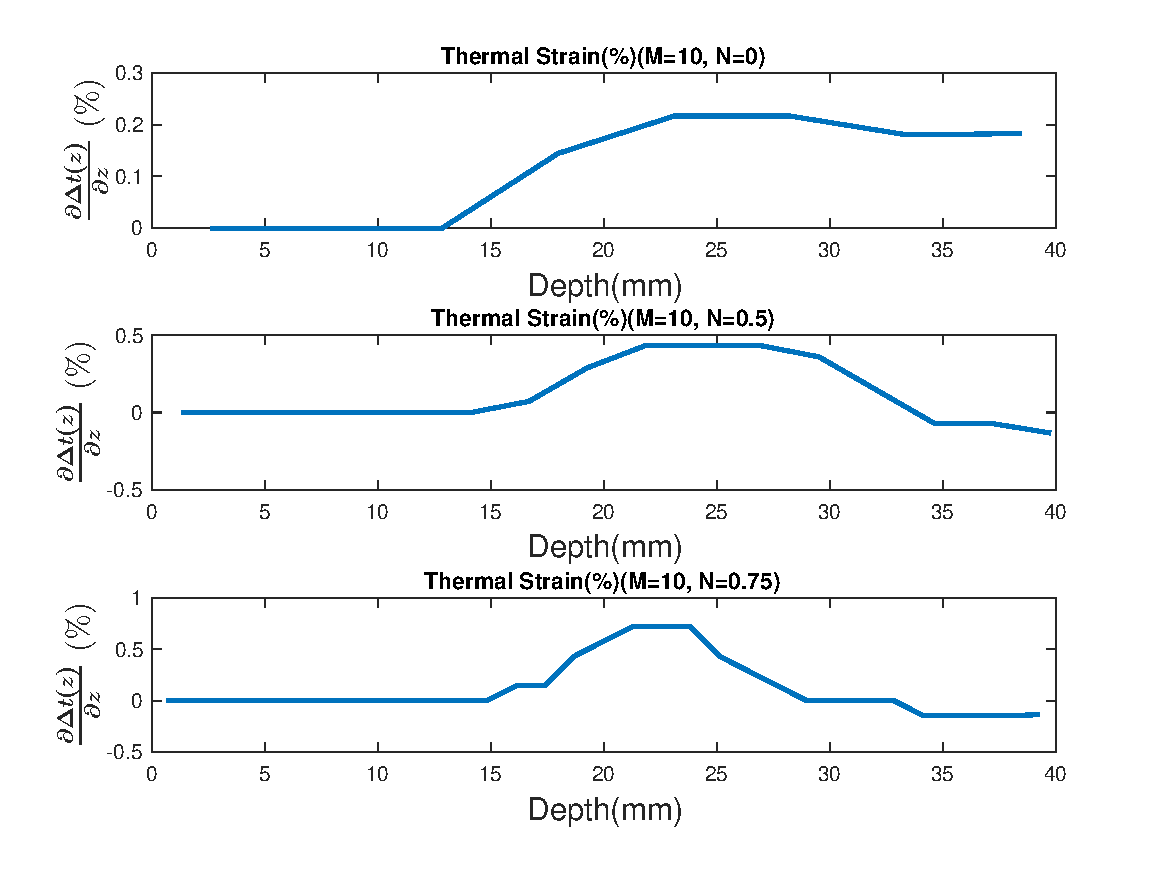
\includegraphics[width=0.82\textwidth]{src/strain_10.pdf}
    \caption{Thermal Strain (M=10)}
    \label{fig:strain-10}
\end{figure}

\end{document}















